\subsection{Task 1 Results}
\label{sec:task1results}
\subsubsection{Geometry and Mesh}
As described in \ref{sec:task1}, simulations have been conducted for the finest mesh size depicted there. Also, after each simulation, the residuals are tracked and checked for convergence. Only then will the results be meaningful in terms of steady-state conditions. For observation, the velocity profiles at the inlet and the outlet are plotted and can be seen from Figure \ref{fig:in_out_comparison}. The velocity profiles are taken from the cross sections that lie on the middle of the straight line segments both at the inlet and outlet. As expected, we see a parabolic shape in both cases with the maximum occurring at the center of the cross section. Also, the mesh used for this experiment can be seen on Figure \ref{fig:mesh}. 

\begin{figure}[H]
    \centering
    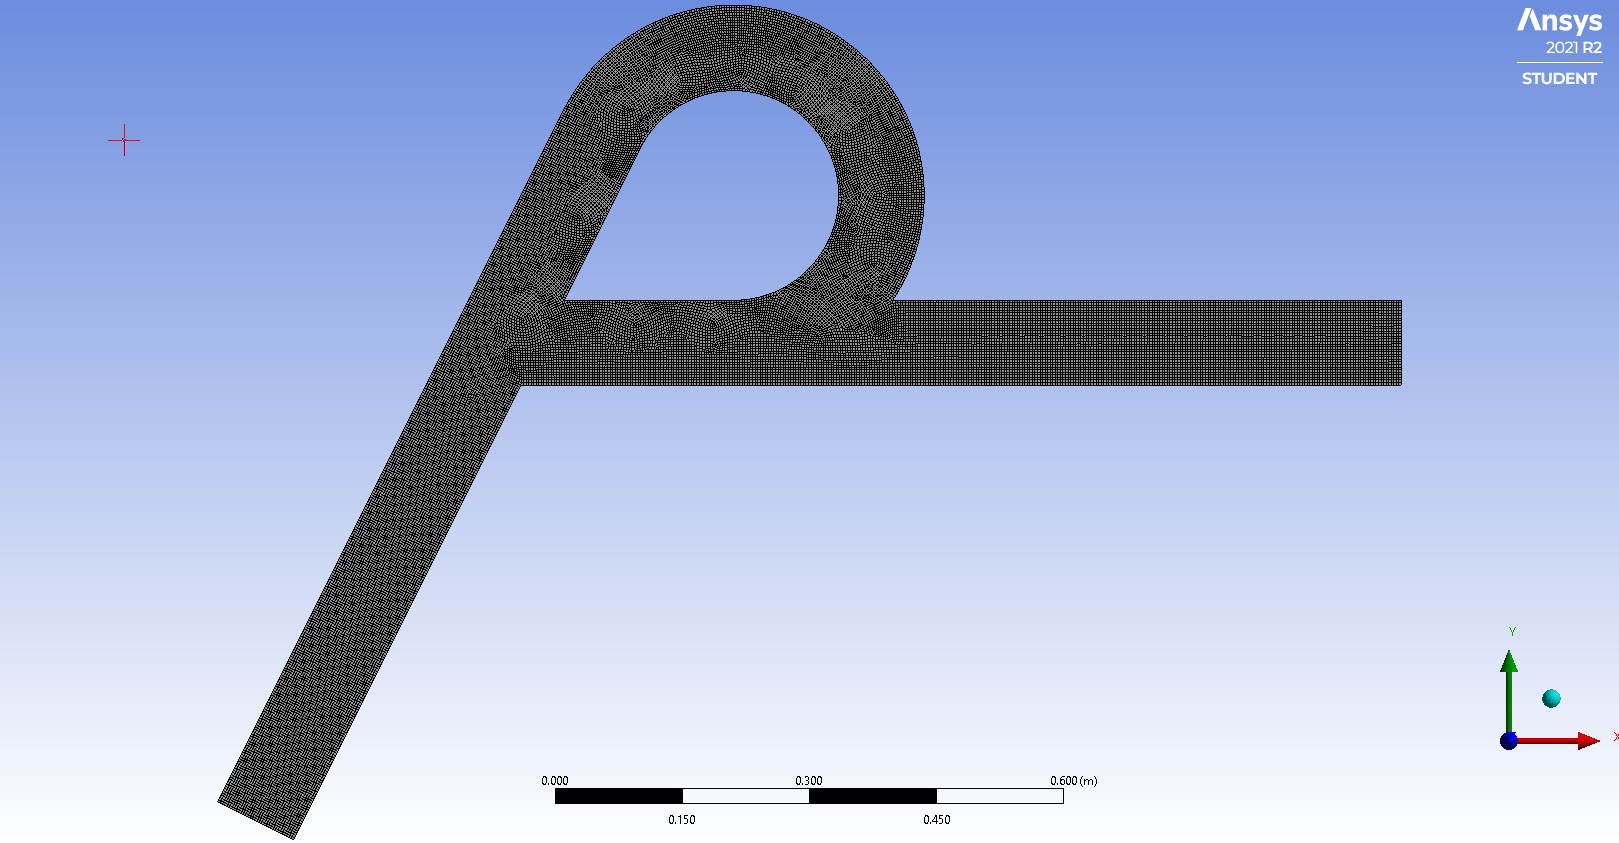
\includegraphics[width=.7\textwidth]{images/task1/3_mesh.png}
    \caption{Sample Mesh}
    \label{fig:mesh}
\end{figure}


\begin{figure}[H]
    \centering
    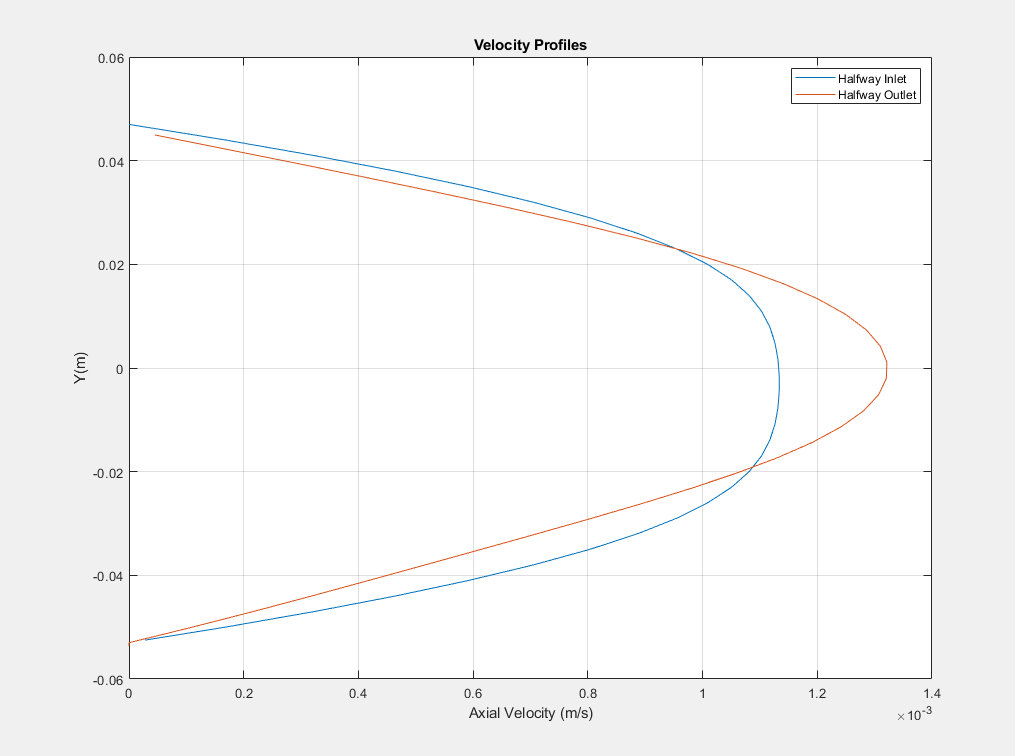
\includegraphics[width=.7\textwidth]{images/task1/3inlet_vs_outlet.png}
    \caption{Comparison of Inlets and Outlets}
    \label{fig:in_out_comparison}
\end{figure}

\subsubsection{Validation}
Further on, to validate our results our computational solutions will be compared with the analytical solutions. For this case, the Couette solution can be applied. The equation for this solution is as follows:
\begin{equation}
    u = 6 * V_{ave} * \Big( \frac{y}{w} - \frac{y^2}{w^2}\Big)
\end{equation}


For validation, the equation is plotted against the ANSYS data we have resulted in, Figure \ref{fig:couette} shows this comparison. As expected, our results agree greatly with the analytical results. For this plot, the ANSYS data are taken from cross sections 75\% into the straight line segments both for the inlet and outlet sections.

\begin{figure}[H]
    \centering
    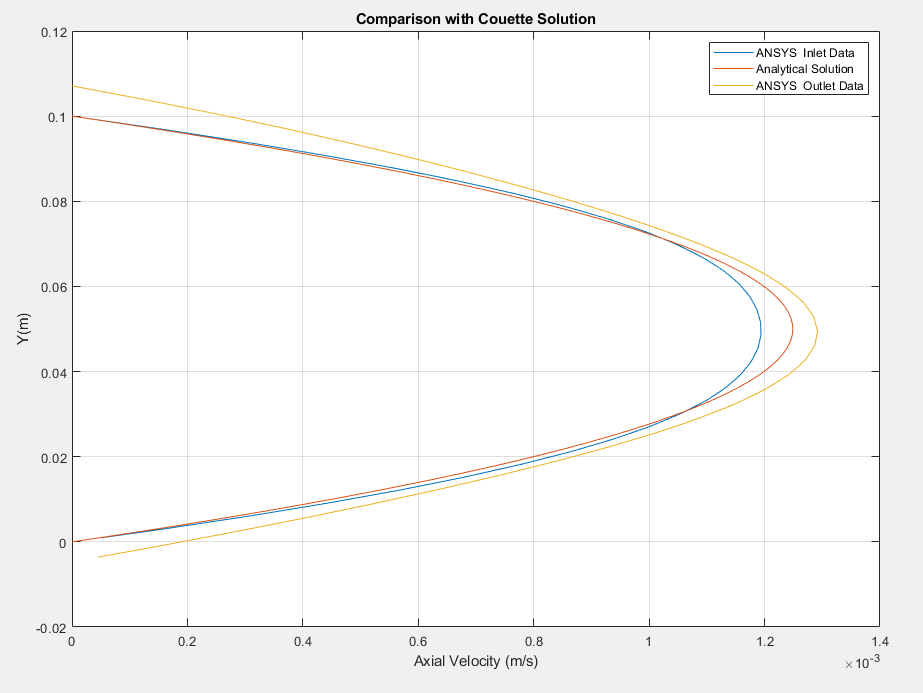
\includegraphics[width=.7\textwidth]{images/task1/couette.png}
    \caption{CFD vs Analytical}
    \label{fig:couette}
\end{figure}


Moreover, various velocity profiles inside are plotted over to demonstrate the development of the boundary layer. Figure \ref{fig:development} shows this plot. The distances from the inlet of those cross sections are as follows:
\begin{itemize}
    \item 10mm
    \item 40mm
    \item 150mm
    \item 225mm
\end{itemize}



\begin{figure}[H]
    \centering
    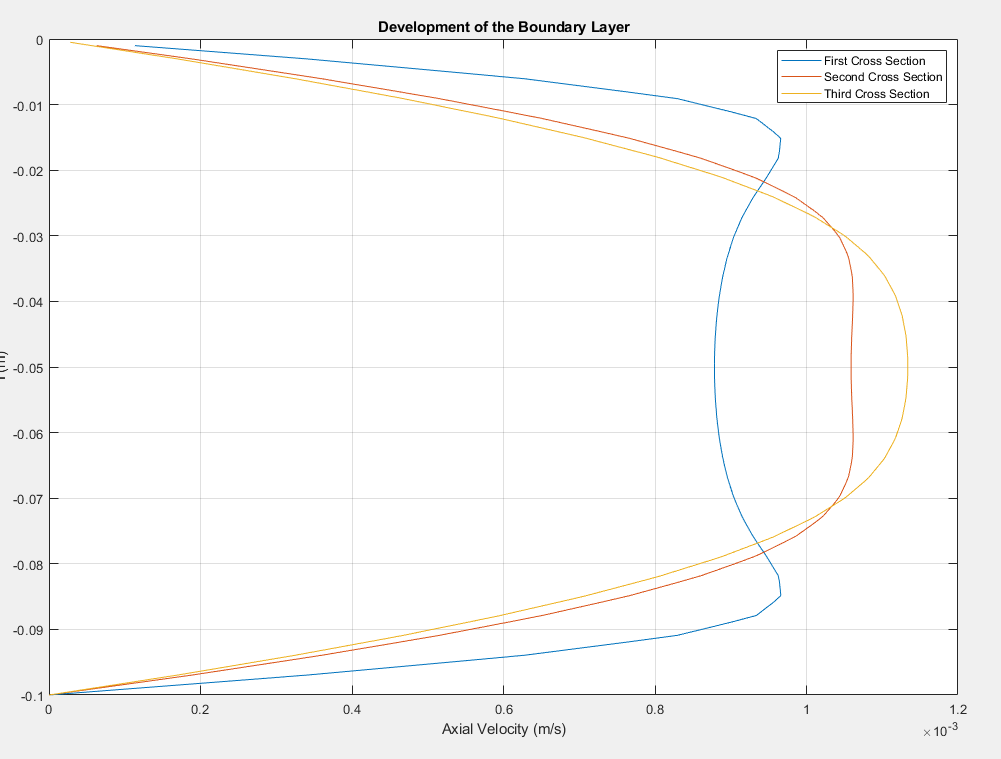
\includegraphics[width=.7\textwidth]{images/task1/development.png}
    \caption{Development of the Boundary Layer}
    \label{fig:development}
\end{figure}

It can be said that the flow develops fully after around the halfway point of the straight line segment. The increased Reynolds number negatively affects the boundary layer. As Re increases, the flow becomes less layered and more unsteady. It can be said that the boundary layer develops earlier for flows with lower Reynolds number. For further information, the pressure contours and streamlines can be found on Figure \ref{fig:press_stream}. 

\begin{figure}[H]
 \centering
\begin{subfigure}{.45\textwidth}
  \centering
  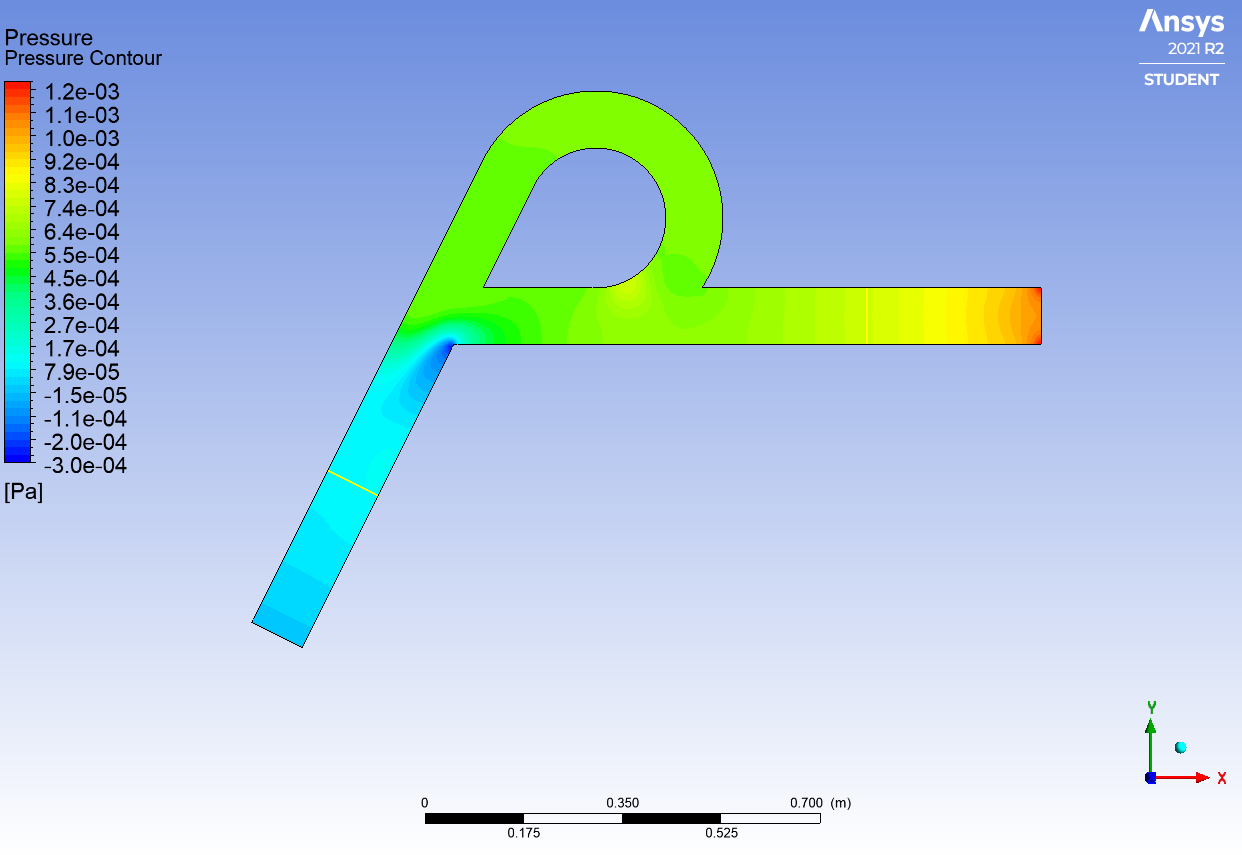
\includegraphics[width=.9\linewidth]{images/task1/6_pressures.png}
  \caption{Pressure Plot for Forward Flow}
  \label{fig:x_d_norm}
\end{subfigure}%
~
\begin{subfigure}{.45\textwidth}
  \centering
  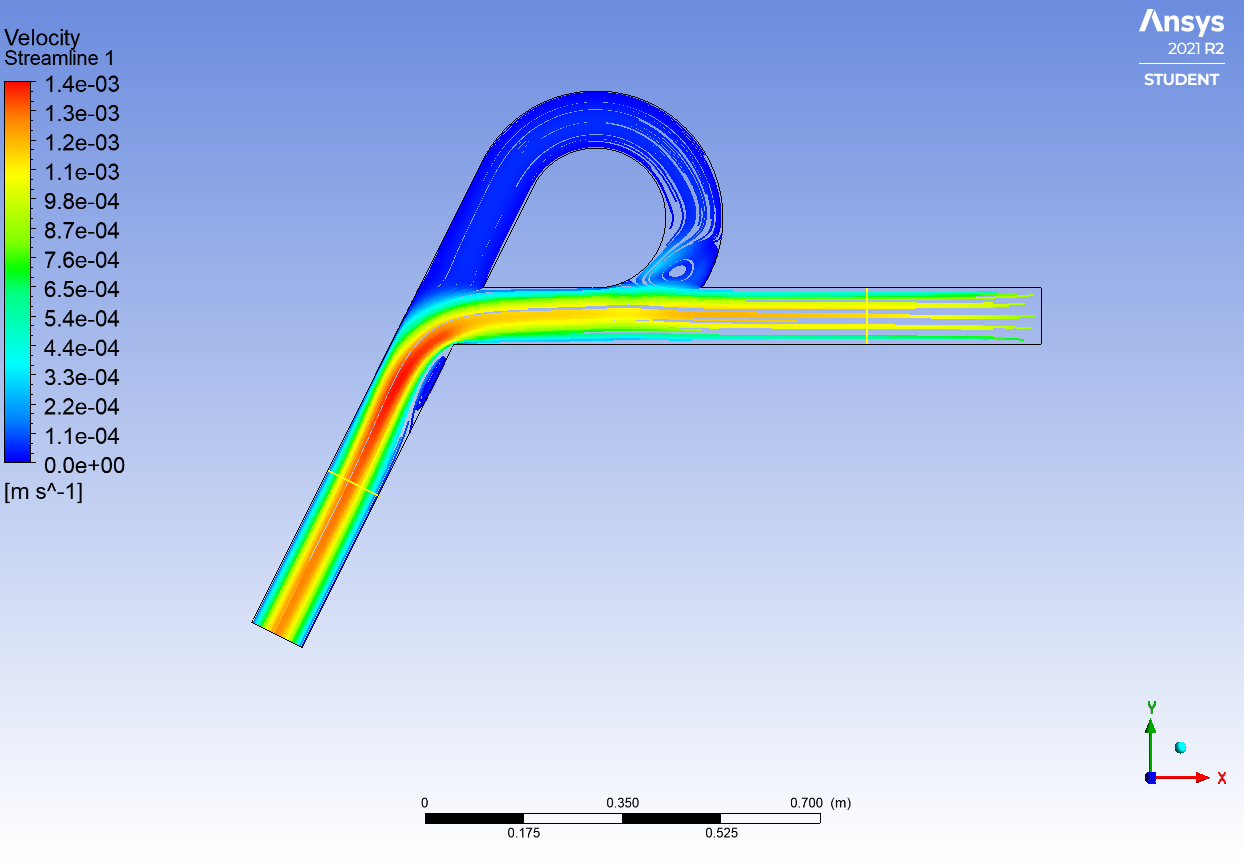
\includegraphics[width=.9\linewidth]{images/task1/6_streamlines.png}
  \caption{Streamlines}
  \label{fig:x_d_norm_actual}
\end{subfigure}
~


\caption{Pressure contours and Streamlines}
\label{fig:press_stream}
\end{figure}